\def\viewA{30}
\def\viewB{45}



% used examples from:
% http://tex.stackexchange.com/questions/212699/text-projection-onto-plane-in-3d-pgf-plots


% Plot planes, that stand for classes of some participants.
%%%%%%%%%%%%%%%%%%%%%%%%%%%%%%%%%%%%%%%%%%%%%%%%%%%%%%%%%%%%%%%%%%%%%%
% 3 coordinates and color
\newcommand{\plotPoint}[4]{
	% the point
	\addplot3[mark=*, color=#4] coordinates { (#1,#2,#3) };	
	
	% projections
	\addplot3[mark=none, dashed, color=#4] coordinates {(0,#2,#3) (#1,#2,#3)};
	\addplot3[mark=none, dashed, color=#4] coordinates {(#1,0,#3) (#1,#2,#3)};
	\addplot3[mark=none, dashed, color=#4] coordinates {(#1,#2,0) (#1,#2,#3)};
}

% Plot planes, that stand for classes of some participants.
%%%%%%%%%%%%%%%%%%%%%%%%%%%%%%%%%%%%%%%%%%%%%%%%%%%%%%%%%%%%%%%%%%%%%%
% 1) participant id; 2) color.
\newcommand{\plotProfPlane}[2]{
	\addplot3[patch,patch type=rectangle, opacity=0.5, color=#2]
		coordinates {(#1,0,0)(#1,5,0)(#1,5,5)(#1,0,5)};
}
% 1) participant id; 2) color.
\newcommand{\plotRoomPlane}[2]{
	\addplot3[patch,patch type=rectangle, opacity=0.5, color=#2]
		coordinates {(0,#1,0)(5,#1,0)(5,#1,5)(0,#1,5)};
}
% 1) participant id; 2) color.
\newcommand{\plotGroupPlane}[2]{
	\addplot3[patch,patch type=rectangle, opacity=0.5, color=#2]
		coordinates {(0,0,#1)(5,0,#1)(5,5,#1)(0,5,#1)};
}




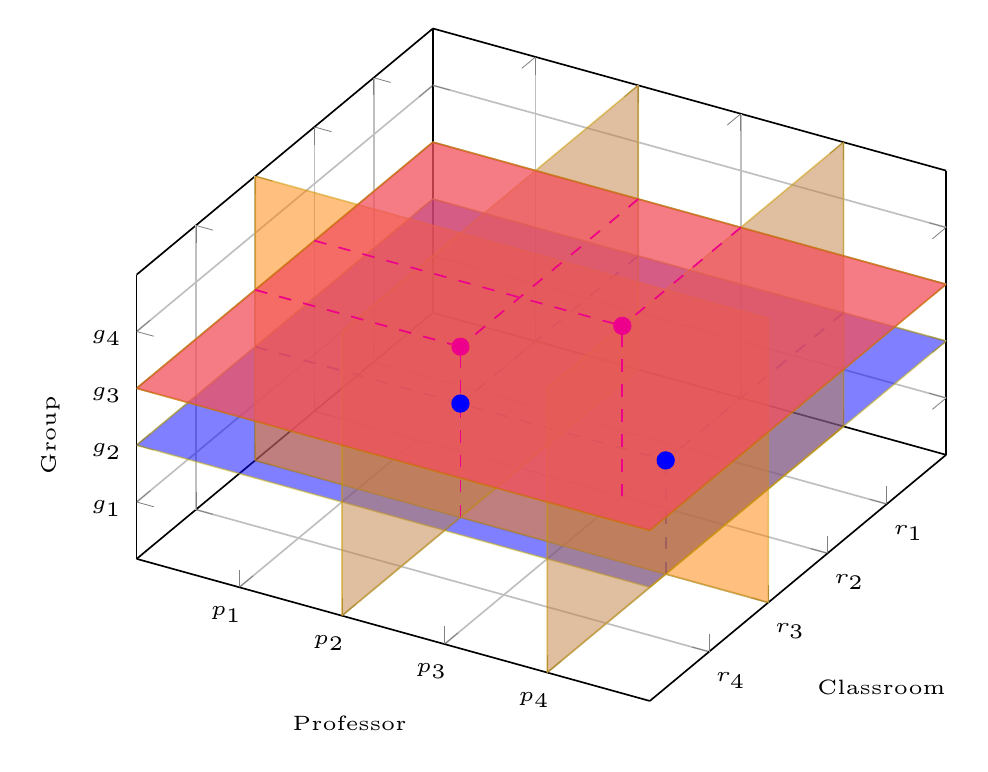
\begin{tikzpicture}[scale=1.5]
\pgfplotsset{every tick label/.append style={font=\tiny}}
\begin{axis}
[
    grid=major,
    view={\viewA}{\viewB},
% X axis
    xmin=0, xmax=5,
    	xlabel = \tiny Professor,
    xtick = {1,2,3,4},
    xticklabel=$p_{\pgfmathprintnumber{\tick}}$,
% Y axis
    ymin=0, ymax=5,
    y dir=reverse,
	ylabel = \tiny Classroom,
    ytick = {1,2,3,4},
    yticklabel=$r_{\pgfmathprintnumber{\tick}}$,	    
% Z axis
    zmin=0, zmax=5,
	zlabel = \tiny Group,
    ztick = {1,2,3,4},
    zticklabel=$g_{\pgfmathprintnumber{\tick}}$,
]

	% 1) let's have a look at g_2 group
	\plotGroupPlane{2}{blue};

	% 2) let's supose it has 2 different sets of classes
	\ifthenelse{\stage > 1}
		{
		\plotPoint{2}{3}{2}{blue};
		\plotPoint{4}{3}{2}{blue};
		}{}

	% 3) within the same classroom r_3
	\ifthenelse{\stage = 3 \OR \stage = 5}
		{
		\plotRoomPlane{3}{orange};
		}{}

	% 4) but with 2 different professors (p_2 and p_4).
	\ifthenelse{\stage = 4}
		{
		\plotProfPlane{2}{brown};
		\plotProfPlane{4}{brown};
		}{}
	% 5) 
	\ifthenelse{\stage = 5}
		{
		\plotGroupPlane{3}{yellow};
		\plotPoint{2}{3}{3}{orange};	
		}{}

	% 6)	
	\ifthenelse{\stage = 6}
		{
		\plotGroupPlane{3}{magenta};
		\plotPoint{2}{3}{3}{magenta};
		\plotPoint{3}{2}{3}{magenta};
		}{}
	
	
\end{axis}
\end{tikzpicture}